\section{Academic Simulation Website}
\label{sec:academicwebsite}
The academic website makes the dual-queue model inspectable through an English-language interface. Users can vary entry arrival rates, class-ending surges, walking assumptions, lift capacities and service cycles, and replay the resulting queues. A fixed seed reproduces a run. The public implementation and source are available online.\footnote{\href{https://liyufei2004.github.io/hku-a2-queue-simulation/}{Live website}; \href{https://github.com/LiYufei2004/hku-a2-queue-simulation}{source repository}.}

\paragraph{Computation and presentation.}
The numerical engine in \texttt{backend/} is separated from controls, animation and plots in \texttt{frontend/}. A versioned Web Worker interface exposes three operations: \texttt{generate} returns replay frames; \texttt{inspect} returns cost components at a selected state; and \texttt{collect} builds conditional tables. The frontend displays returned values rather than independently implementing the choice equations. Workers keep computation off the main interface thread; a separate collection worker allows replay inspection during table generation. Static GitHub Pages hosting is sufficient, without an HTTP application server or database. This website backend is JavaScript, distinct from any separately developed team SimPy implementation.

\paragraph{Observation and explanation.}
Replay distinguishes physical queues from people walking to their chosen destination. A passenger joins a queue only on reaching its tail, and boarding follows individual lift events. Inspection separates walking time, expected position loss and batch-service waiting time. It explains why a shorter-looking queue can remain unattractive once switching costs are included. The corridor drawing is illustrative, rather than evidence of measured pedestrian geometry.

\paragraph{Partial-information lookup.}
The lookup conditions on entry side, time window and observed local queue length to estimate the opposite queue's empirical distribution. It compares conditional mean costs using the same cost function as the full-information engine, without inspecting the hidden live queue. Missing conditions remain missing, and fewer than 30 matching snapshots produces no definite recommendation. Changing parameters invalidates the table. CSV/JSON exports preserve parameters, seed, bins, counts and cost sums for reproducibility.

\begin{center}
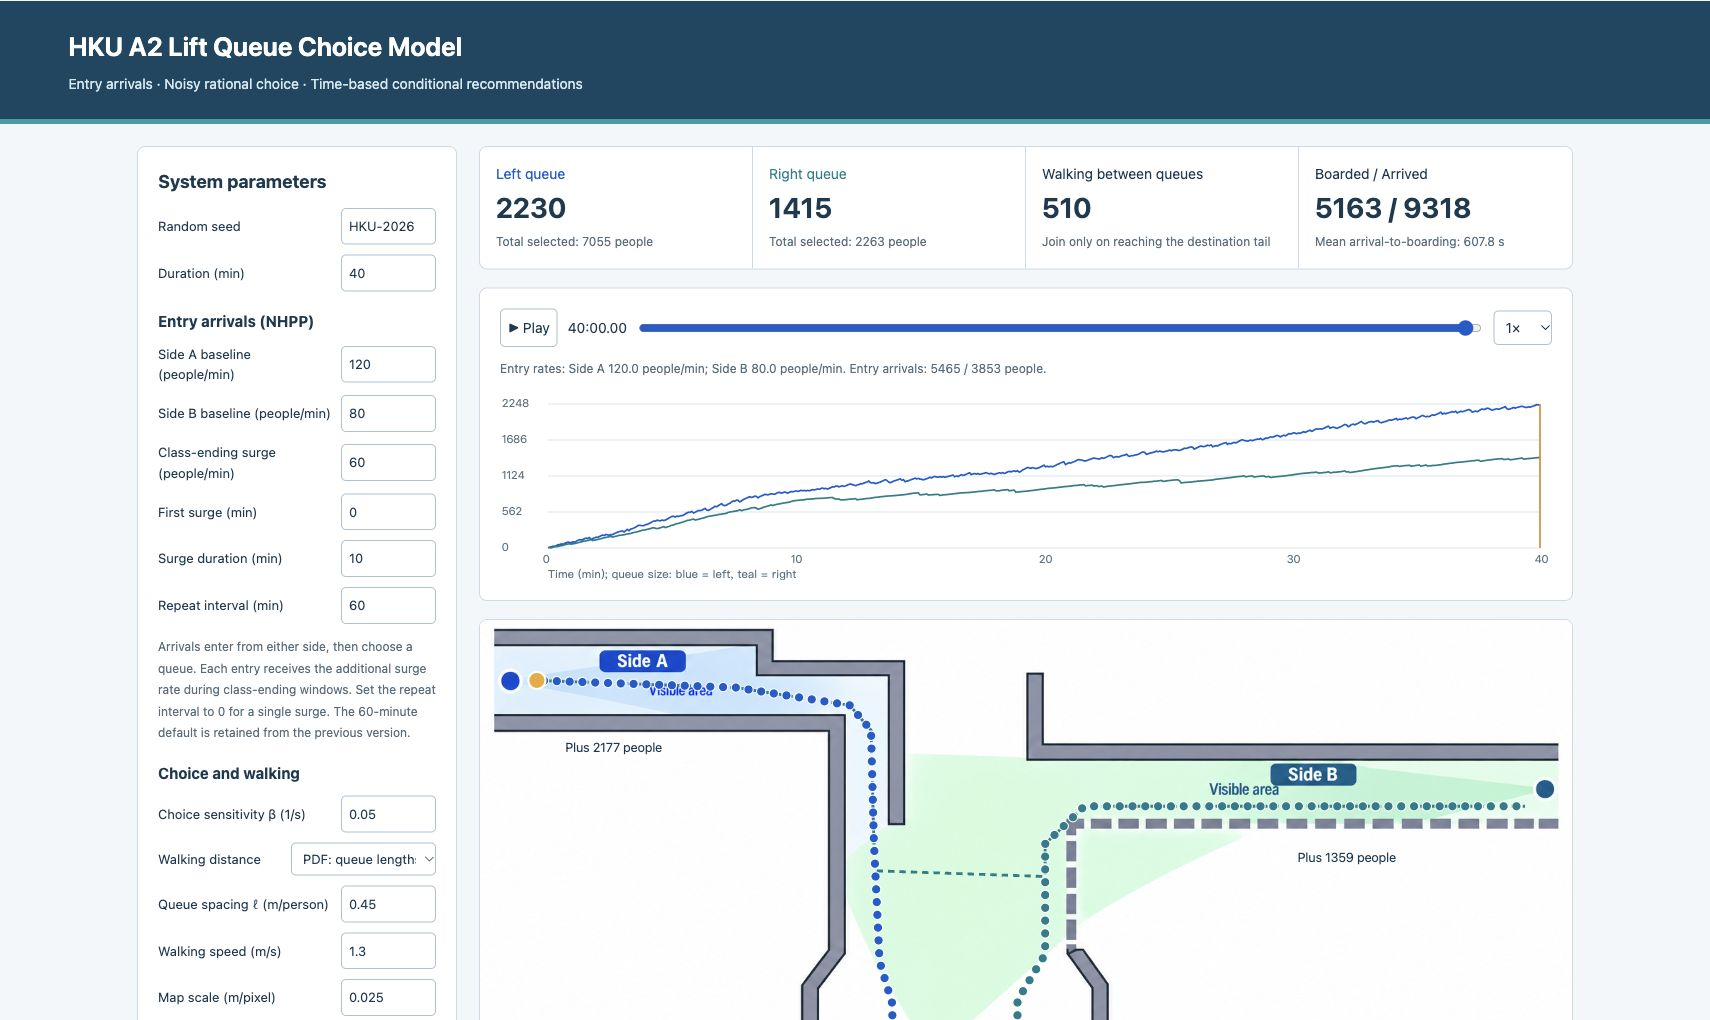
\includegraphics[width=.9\linewidth,height=5.3cm,keepaspectratio]{figures/website_overview.png}
\captionof{figure}{Local website replay with illustrative default inputs. Queue counts and displayed delays are simulated, not field measurements.}
\end{center}
